\documentclass[12 pt, a4paper]{article} %E aceptable tamen 11pt
%\usepackage[galician]{babel}\decimalpoint  %Para Galego
\usepackage[spanish]{babel}  %Para Castelan
%\usepackage[english]{babel}\decimalpoint    %Para Ingles
\usepackage[utf8]{inputenc} %acentos e caracteres para Windows & Linux         
\usepackage[T1]{fontenc}
\usepackage{graphicx}
\usepackage{color}
\usepackage{tikz}
\usepackage{anysize}
\usepackage{multicol}
\usepackage{bm}
\usepackage{textcomp}
\usepackage{eurosym}
\usepackage{amsthm}
\usepackage{amsmath}
\usepackage{amsfonts}
\usepackage{amssymb}
\usepackage{lineno}
\usepackage{epstopdf}
\usepackage{fancyhdr}
\usepackage{subfigure}
\usepackage{float}
\usepackage[square, numbers]{natbib}
\usepackage{longtable}
\usepackage{multirow}
\usepackage{array}
\usepackage{tabularx}
\usepackage[linkcolor=blue,colorlinks,]{hyperref}
%\usepackage{lipsum}
\usepackage{mathdots}
\usepackage{braket}
\usepackage{yhmath}
\usepackage{cancel}
%\usepackage{siunitx}
\usepackage{gensymb}
\usepackage{booktabs}

\usetikzlibrary{fadings}
\usetikzlibrary{patterns}

\parindent=0mm %sangría
\parskip=3mm   %separacion entre parrafos
\usepackage{gensymb}

\numberwithin{equation}{section}
\numberwithin{figure}{section}

\renewcommand{\spanishtablename}{Tabla} %Denominacion para tablas
\renewcommand{\spanishabstractname}{} %Denominacion para el abstract
\renewcommand{\spanishrefname}{Referencias} %Denominacion para las referencias
\renewcommand{\spanishfigurename}{Figura} %Denominacion para imagenes
\renewcommand{\spanishchaptername}{} %Denominacion para capitulos
\renewcommand{\spanishcontentsname}{Índice} %Denominacion para el indice


\definecolor{usc}{RGB}{15,41,118}
\definecolor{grise}{RGB}{234, 236, 240}
\newcommand{\abs}[1]{\lvert#1\rvert}

\newcommand{\vect}[1]{\boldsymbol{\mathbf{#1}}}


\begin{document}
	\pagenumbering{Roman}
	%%%%%%%%%%%%%%%%%%%%%%%%%%%% TITULO %%%%%%%%%%%%%%%%%%%%%%%%%%%%%%%%%%%%%%%%%%%%%%%%%%%%%%%
	\pagestyle{empty}
	
	\newcommand\TituloDoTraballo{Caracterización de la emisión en radio en cascadas atmosféricas iniciadas por
		neutrinos tau de muy altas energías en detectores a gran altitud}  % <-- Titulo tal como vai aparecer na portada externa e na interna. Debe coincidir co titulo subido a secretaria virtual no momento do deposito da memoria/solicitude de defensa. Non ten por que coincidir co titulo do proxecto do traballo (o titor debe incluir no seu informe o seu acordo co titulo final). O mais adecuado e que o titulo na portada este no idioma do texto principal da memoria. Tamen pode cambiarse de idioma do resto do contido da portada.
	
	\newcommand\EspecialidadeMaster{Especialidad en Física Nuclear y de Partículas}  % <-- Deixar valeiro no caso de TFG, e decir introducir {}. No caso de TFM, e IMPORTANTE que conste: Esta considerado un requisito para obter a especialidade da titulacion do master que a devandita especialidade conste no TFM,  sucedendo que na implementacion informatica da USC ao facer a solicitude de defensa de TFM na secretaria virtual a unica opcion onde introducir a especialidade e no propio campo do titulo do traballo. Por eso, a mencion de especialidade debe facerse como unha addenda ao titulo de TFM, a modo de subtitulo - en particular, na secretaria virtual, este subtitulo ou mencion a especialidade debe incluirse no mesmo campo informatico do titulo de TFM (por exemplo introducir no campo titulo do TFM "Estudio de superconductores ultrarelativistas. Especialidad en Fisica Fundamental." Asi vai aparecer tamen no expediente academico do estudante.)
	
	\newcommand\DataDefensa{Junio 2022} %<-Mes e ano da presentacion
	
	\begin{center}
		%{\sc\large\color{usc} \sc Universidade de Santiago de Compostela}
		\vspace{3em}
		
\includegraphics[width=10em]{figures/USC.png}
		\hspace{1cm}
		\begin{tabular}[b]{c}
			{\large\color{usc} \sc Facultad de Física} \vspace{0.5em}\\
			{\large\color{usc} \sc Grado en Física } \vspace{0.5em}\\  %<-- Ou Master
			{\large\color{usc}  Curso 2021-22} \vspace{0.5em}\\%Actualizar curso!
			{\Large\color{usc} \sc Trabajo de Fin de Máster} %<-- Ou Master
		\end{tabular}
		
		
		
		\vspace{3cm}
		\rule{65mm}{0.2mm}\\
		\vspace{1cm}
		
		{\sc\LARGE \TituloDoTraballo}
		
		{\sl\large \EspecialidadeMaster}
		
		
		
		\vspace{0.5cm}
		\rule{65mm}{0.2mm}\\
		\vspace{2cm}
	\end{center}
	
	
	\begin{tabular}{l}
		{\sl\large Autor:} \\
		{\bf\Large Sergio Cabana Freire} % nome e apelidos do estudante
		\vspace{1em}\mbox{} \\
		%
		{\sl\large Tutor:} \\
		{\bf\large Jaime Álvarez Muñiz} \\
		{\sl\large Departamento de Física de Partículas \& IGFAE}
		\vspace{1em}\mbox{} \\
		%
	\end{tabular}
	
	
	
	\mbox{}
	\mbox{}\hfill{\large \DataDefensa} \vspace{1cm}
	
	\noindent{\tiny El autor autoriza la consulta y empleo de esta memoria para uso acad\'emico y de investigaci\'on (autorizaci\'on detallada en las p\'aginas interiores).}
	
	
	
	\clearpage
	\mbox{}
	\clearpage %fin portada externa, inicio portada interna%%%%%%%%%%%
	
	\mbox{}\\
	Facultad de F\'{\i}sica\\
	Grado en F\'{\i}sica \\  
	Curso 2021-22\\%Nota: actualizar curso
	{\sc Trabajo de Fin de Máster}\vspace{3cm}\\
	%
	{\sc\LARGE \TituloDoTraballo}\vspace{1cm}\\
	{\sl\large \EspecialidadeMaster}\vspace{2cm}\\
	%
	{\sl Autor:} {\bf Sergio Cabana Freire}\\ % nome e apelidos do estudante
	{\sl Tutor:} {\bf Jaime Álvarez Muñiz}, {\sl Departamento de Física de Partículas (USC) \& Instituto Galego de Física de Altas Enerxías (IGFAE)}\\
	\vspace{1cm}\\
	%
	%Opcionalmente, inclu\'{\i}r aqu\'{\i}  li\~nas de agradecementos a outras persoas que colaborasen, referencias a financiaci\'on econ\'omica, notas sobre patentes ou publicaci\'ons de traballos derivados do traballo, ou calqueira outra informaci\'on complementaria de contextualizaci\'on xeral do traballo que considere convinte.
	
	\mbox{}
	
	\mbox{}\hfill{Data de presentaci\'on: \DataDefensa}
	
	
	\clearpage
	%%%%%%%%%%%%%%%%%%%%%%%%%%%%%%%%%%%%%%%%%%%%%%%%%%%%%%%%%%%%%%%%%%%%%%%%%%%%%%%%%
	
	%%%%%%%%%%%%%%%%%%%%%%%%%%%%%%%%%%% DECLARACIONES %%%%%%%%%%%%%%%%%%%%%%%%%%%%%%%
	\thispagestyle{empty}
	\pagebreak
	
	{\sl Declaraci\'on firmada por el autor de la originalidad del trabajo}
	
	El autor del trabajo declara que e presente es un trabajo original. Autoriza asimismo al control por personal de la Universidade de Santiago de Compostela de la mencionada originalidad, eventualmente mediante el empleo de bases de datos y la inclusi\'on en ellas.
	
	En Santiago de Compostela, a X de junio de 2022. Firmado,\vspace{3cm}
	
	
	{\sl Autorizaci\'on del autor a la difusi\'on del trabajo}
	
	 El autor autoriza a la difusi\'on del trabajo a los efectos considerados en los vigentes reglamentos de TFG y TFM de la Universidade de Santiago de Compostela (Artículo 11.3) y de TFM del M\'aster en F\'{\i}sica (Artículo 33), entendiendo que esta autorizaci\'on no infl\'uye en la propiedad intelectual del trabajo ni a la posibilidad de publicar el mismo total o parcialmente por otros medios. Autoriza asimismo a que la Facultad de F\'{\i}sica de esa Universidad disponga de copia electr\'onica del trabajo para su archivo, consulta y empleo para usos acad\'emicos y de investigaci\'on con la menci\'on espec\'{\i}fica al autor. 
	
	En Santiago de Compostela, a X de junio de 2022. Firmado,\
	
	\thispagestyle{empty}
	\pagebreak
	%%%%%%%%%%%%%%%%%%%%%%%%%%%%%%%%%%%%%%%%%%%%%%%%%%%%%%%%%%%%%%%%%%%%%%%%%%%%%%%%%

	%%%%%%%%%%%%%%%%%%%%%%%%%%%%%%%%%%%%%%%% ABSTRACTS %%%%%%%%%%%%%%%%%%%%%%%%%%%%%%%%%%
	\thispagestyle{empty} %%<- poner en mas paginas si los resumenes ocupan varias (elimina la numeracion de la pagina actual)
	\pagebreak
	
		\begin{flushleft} \hyphenpenalty=10000\exhyphenpenalty=10000 {\bf $\bullet$ Resumen:\;\;}
		%
		Aqu\'{\i} va el resumen en castellano. El orden de los idiomas puede cambiarse a voluntad. Tambi\'en (y aunque la hoja de res\'umenes no contabiliza para el n\'umero l\'{\i}mite de p\'aginas, ver secci\'on \ref{quecontabiliza} de este documento) puede  reducirse, si se desea, el tama\~no de letra de los res\'umenes en los dos idiomas que no sean el usado  en el texto principal de la memoria (por ejemplo, anteponiendo \verb \footnotesize{}  al texto). % anteponiendo \footnotesize{} al texto, por ejemplo
		%
	\end{flushleft}\mbox{}

	\begin{flushleft} \hyphenpenalty=10000\exhyphenpenalty=10000 {\bf $\bullet$ Resumo:\;\;}
		%
		Aqu\'{\i} vai o resumo en galego. Debe coincidir co introducido na secretar\'{\i}a virtual no momento do dep\'osito da memoria final e solicitude de defensa. Dado que a aplicaci\'on inform\'atica de secretar\'{\i}a virtual non admite calqueira caracter, o regulamento permite introducir nela representaci\'ons alternativas dos caracteres problem\'aticos (por exemplo introducir gamma en vez de $\gamma$, introducir YBa2Cu3O(7-delta) en vez de \mbox{YBa$_2$Cu$_3$O$_{7-\delta}$}, etc.). Non ten por qu\'e coincidir co resumo do proxecto de TFG/TFM que foi feito no momento da asignaci\'on de traballo e titor (entendendo que o titor da o visto bo no seu informe final). Ten que haber resumos en (como m\'{\i}nimo) galego, castel\'an e ingl\'es, cada un de 300 palabras m\'aximo.
		%
	\end{flushleft}\mbox{}
	
	
	\begin{flushleft} \hyphenpenalty=10000\exhyphenpenalty=10000 {\bf $\bullet$ Abstract:\;\;}
		%
		The abstract goes here.
		%
	\end{flushleft}\mbox{}
	%%%%%%%%%%%%%%%%%%%%%%%%%%%%%%%%%%%%%%%%%%%%%%%%%%%%%%%%%%%%%%%%%%%%%%%%%%%%%%%%%%%%%
	%\clearpage
	%\include{capitulos/resumo} % paxina de resumo e agradecementos. Débese ter en conta o idioma seleccionado para o documento
	
	\clearpage
	\pagestyle{fancy}
	\fancypagestyle{plain}
	\lhead{}
	\chead{}
	\rhead{}
	\renewcommand{\headrulewidth}{0.1pt}
	\lfoot{} 
	\cfoot{\thepage}
	\rfoot{} 
	\renewcommand{\footrulewidth}{0pt}
	
	\pagenumbering{arabic}\setcounter{page}{1}
	\tableofcontents
	\clearpage
	
	%%%%%%% Incluimos as seccións que sexan necesarias
	\section{Introducción}
	\clearpage
	\section{Emisión en radio: Principio físico y caracterización}
	El objetivo fundamental de este trabajo, como hemos comentado en el apartado introductorio, es la caracterización de las radiofrecuencias emitidas en cascadas atmosféricas y el estudio de su posible aprovechamiento para la detección de neutrinos tau de origen astrofísico. Para poder avanzar en esta cuestión, debemos plantear los mecanismos físicos que originan dicha emisión, ya que una buena comprensión de los mismos es, como poco, importante para poder interpretar los resultados posteriores.
	\subsection{Formalismo de la emisión}
	Como es bien sabido, la presencia de cargas en movimiento en un determinado medio implica, casi de manera inevitable, la emisión de radiación electromagnética. Resulta entonces evidente que, en una cascada atmosférica iniciada, por ejemplo, por un protón o un neutrino de origen astrofísico en la que aparecerán un número gigantesco de partículas cargadas propagándose con una velocidad $v\sim c$, podemos esperar la aparición de radiación electromagnética.
	
	Ahora bien, uno podría pensar de manera ingenua que, en las escalas de energía y número de partículas que involucra una cascada atmosférica, el balance \textit{macroscópico} de cargas positivas y negativas debería ser nulo, y por lo tanto las respectivas contribuciones a la radiación electromagnética emitida deberían cancelarse. Sin entrar en demasiado detalle, basta recordar que los potenciales electromagnéticos pueden expresare como:
	\begin{equation}
		\Phi(\vect{r}, t) \propto \int_{\text{fuente}} \frac{\rho\left(\vect{r}', t_{ret}\right)}{\left|\vect{r}-\vect{r}'\right|}d^3r'\;\;;\;\;\vect{A}(\vect{r}, t)\propto\int_{\text{fuente}} \frac{\vect{J}\left(\vect{r}', t_{ret}\right)}{\left|\vect{r}-\vect{r}'\right|}d^3r' \label{ec21}
	\end{equation}
Si uno toma que, en promedio, $\langle\rho\rangle\sim0$ y $\langle\vect{J}\rangle\sim0$, no cabría mucha opción para detectar radiación electromagnética a partir de una cascada atmosférica.

Evidentemente, esta situación desaparece inmediatamente cuando tenemos en cuenta que la cascada se desarrolla en presencia del campo magnético terrestre, y por lo tanto las cargas sufren una deflexión en un sentido u otro según el signo de su carga. En la perspectiva \textit{macroscópica}, podemos interpretar que este efecto de deflexión geomagnética origina una corriente neta perpendicular tanto al desarrollo de la cascada como al campo magnético terrestre, generando entonces un campo eléctrico $\vect{E}=-\dot{\vect{A}}$

\begin{figure}[H]
	\centering
	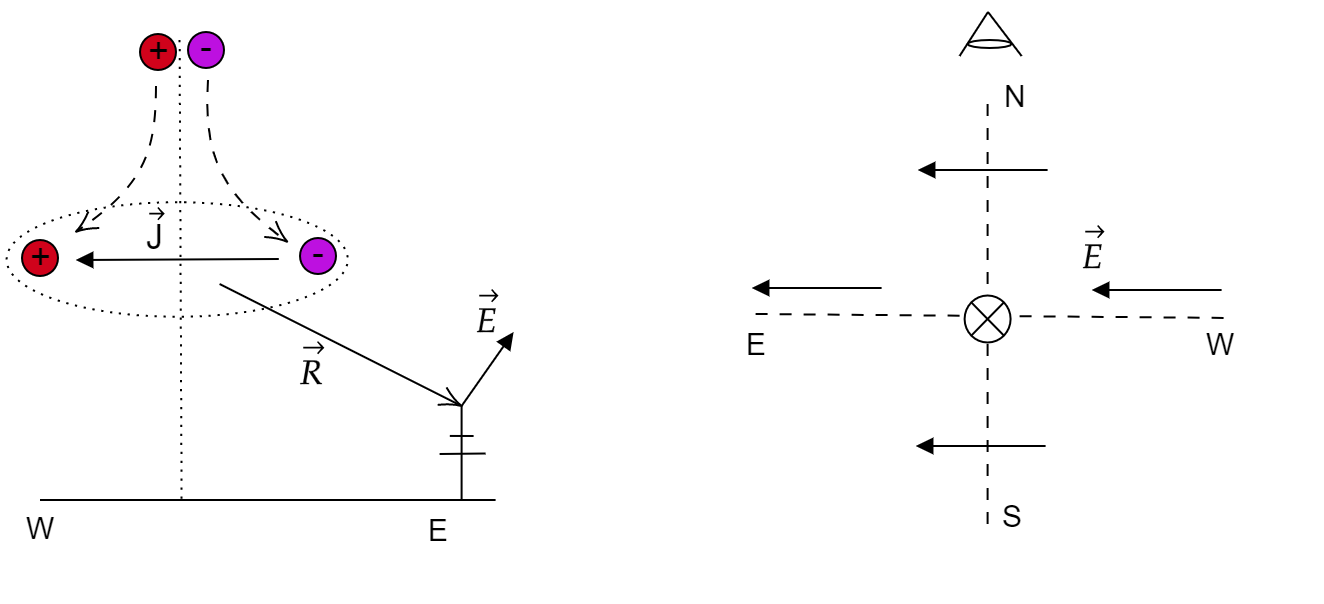
\includegraphics[width=0.8\linewidth]{figures/Geomag_deflexion}
	\caption{Imagen macroscópica del campo eléctrico generado debido a la deflexión geomagnética, para una cascada vertical. De manera muy simplificada, $\vect{E}=-\dot{\vect{A}}\parallel -\vect{J}$. Las direcciones N, S, E, W son relativas al polo norte magnético.}
	\label{Geomag_deflexion}
\end{figure}
	\subsection{Caracterización de la emisión en simulaciones Monte Carlo}
	\clearpage
	\section{Caracterización de cascadas hacia arriba}
	\clearpage %cleardoublepage pode meter paxinas en branco. Non e obrigatorio. Tampouco para a 
	\section{Emisión en radio en cascadas hacia arriba}
	\clearpage %cleardoublepage pode meter paxinas en branco. Non e obrigatorio. Tampouco para a 
	\section{Conclusiones}
	
	
	%%%%%%%Bibliografía
	\clearpage
	\appendix
	\markboth{REFERENCIAS}{REFERENCIAS}  
	\addcontentsline{toc}{section}{Referencias} 
	\nocite{*}
	\bibliography{TFMbib}
	\bibliographystyle{apalike}

	
\end{document}